\begin{frame}[fragile]{Client analyses}
    We validate \intrajs\ by implementing three different dataflow analyses:
    \begin{itemize}\small
        \item {\color<2->{ForestGreen}{\texttt{NullPointerAnalysis}}} - \emphSlide{NPA} \hfill \textbf{MAY - FORWARD }
        \item \texttt{LiveVariableAnalysis} - \emphSlide{LVA} \hfill \textbf{MAY - BACKWARD}
        \item \texttt{DeadAssignmentAnalysis} - \emphSlide{DAA} \hfill uses \emphSlide{LVA}
    \end{itemize}
\vspace{0.5cm}
\hspace{-0.8cm}
	    \begin{minipage}[h]{0.4\textwidth}
\onslide<2->{
	     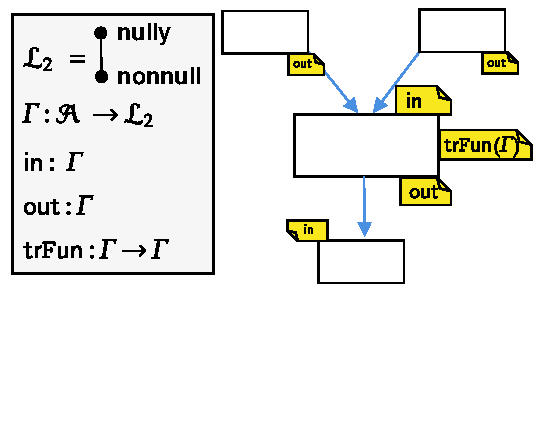
\includegraphics[scale=0.65]{img/npa.pdf}%
}
    \end{minipage}\hfill%
	    \begin{minipage}[h]{0.5\textwidth}
\begin{onlyenv}<3->


\footnotesize
$\bullet$\ Default behaviour for \texttt{CFGNodes}
\begin{lstlisting}[frame=none,language=JastAdd]
trFun(@$\Gamma$@){
  return @$\Gamma$@;
}
\end{lstlisting}
 $\bullet$\ Specialised behaviour for \texttt{AssignExpr}
\begin{lstlisting}[frame=none, language=JastAdd]
trFun(@$\Gamma$@){
  if(rhs.mayBeNull())
    @$\Gamma$@.put(lhs.decl(),nully);
  else
    @$\Gamma$@.put(lhs.decl(),nonnull);
  return @$\Gamma$@;
}
\end{lstlisting}

\end{onlyenv}
    \end{minipage}%

\end{frame}
%\begin{frame}{Overview}
%We conducted two different studies:\vspace{0.2cm}
%	\begin{itemize}
%		\item We compared the size of the CFGs constructed by \intrajs\ against the ones constructed by the earlier  RAG-based framework \lowEmph{Jastaddj-intraflow} (JJI)\vspace{0.1cm}
%
%		\item We compared the precision and performance of \intrajs\  against the highly-tuned  industrial static checker \lowEmph{SonarQube} (SQ)
%
%	\end{itemize}
%
%\onslide<2->{
%\begin{table}
%\centering
%\begin{tabular}{l|l|l|l|l}
%     & \textsc{Antlr}                    & \textsc{Pmd}                      & \textsc{Jfc}                      & \textsc{Fop}                      \\
%\hline
%\textsc{LOC}  & \multicolumn{1}{c|}{33K} & \multicolumn{1}{c|}{49K} & \multicolumn{1}{c|}{95K} & \multicolumn{1}{c}{97K}
%\end{tabular}
%\end{table}
%}
%\end{frame}

\begin{frame}{Overview}
\begin{center}
\only<1>{%

\includegraphics[scale=0.7]{img/eval1.pdf}%
}%
\only<2>{%

\includegraphics[scale=0.7]{img/eval15.pdf}%
}%
\only<3>{%
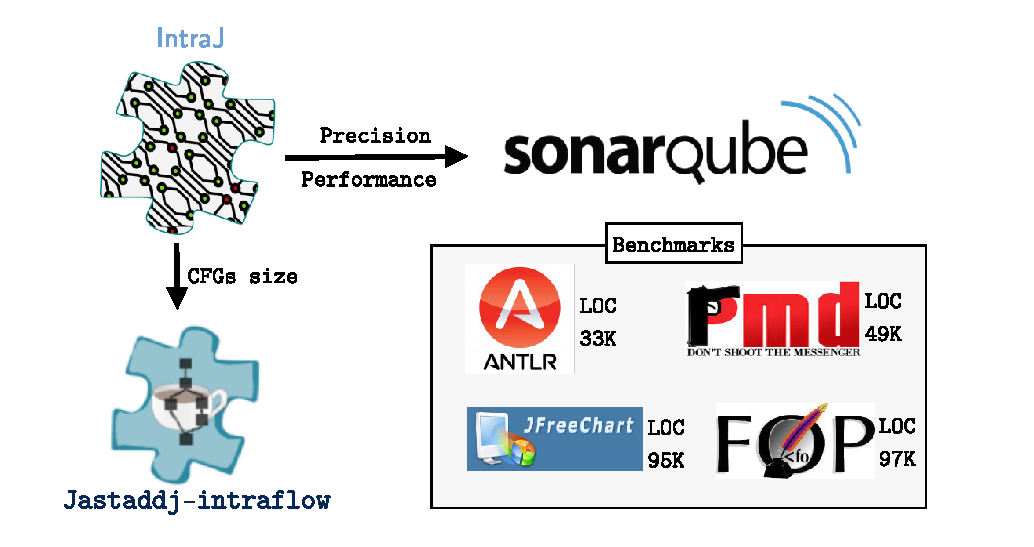
\includegraphics[scale=0.7]{img/eval2.pdf}%
}%
\end{center}
\end{frame}


\begin{frame}[fragile]{Benchmark Projects}
\begin{center}
  \intrajs\ reduces the CFGs  size by 30\% - 40\%
  \begin{table}
\centering
\begin{tabular}{ccccc}
Benchmark & Qty & \intraj& JJI & \% \\
\hline
\multirow{2}{*}{\textsc{Antlr}} & \textsc{Nodes} & 76$^\cdot$925 & 116$^\cdot$523 & \emphSlide{-39.9} \\
\cline{2-5}
 & \textsc{Edges} & 85$^\cdot$028 & 136$^\cdot$528 & \emphSlide{-37.7} \\
\hline
\multirow{2}{*}{\textsc{Pmd}} & \textsc{Nodes} & 103$^\cdot$739 & 182$^\cdot$864 & \emphSlide{-43.2} \\
\cline{2-5}
 & \textsc{Edges} & 108$^\cdot$639 & 202$^\cdot$842 & \emphSlide{-46.4} \\
\hline
\multirow{2}{*}{\textsc{Jfc}} & \textsc{Nodes} & 219$^\cdot$419 & 331$^\cdot$368 & \emphSlide{-33.7} \\
\cline{2-5}
 & \textsc{Edges} & 220$^\cdot$256 & 363$^\cdot$642 & \emphSlide{-39.4} \\
\hline
\multirow{2}{*}{\textsc{Fop}} & \textsc{Nodes} & 239$^\cdot$096 & 347$^\cdot$125 & \emphSlide{-31.1} \\
\cline{2-5}
 & \textsc{Edges} & 240$^\cdot$068 & 379$^\cdot$269 & \emphSlide{-36.6} \\
\hline
\end{tabular}
\end{table}
By removing all the {\color{orange}redundant} nodes
\end{center}
\end{frame}



\begin{frame}[fragile]{\intrajs\  vs \lowEmph{SonarQube}}
	We evaluated \emphSlide{IntraJ} against \lowEmph{SonarQube}
		\only<1>{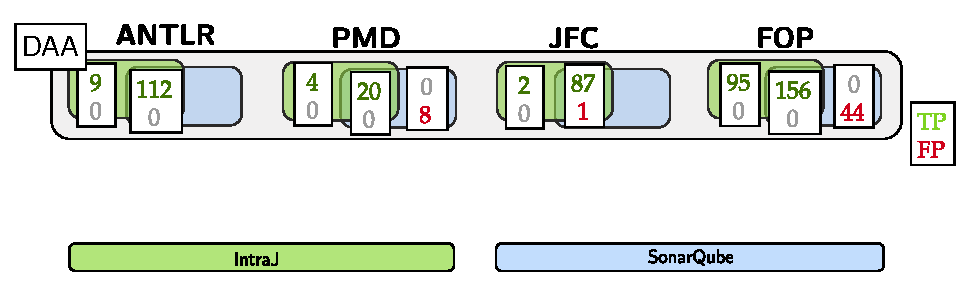
\includegraphics[scale=0.7]{img/precision1.pdf}}
		\only<2>{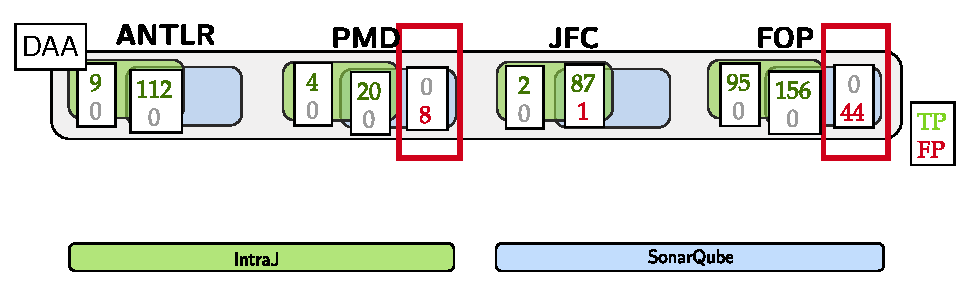
\includegraphics[scale=0.7]{img/precision2.pdf}}
		\only<3>{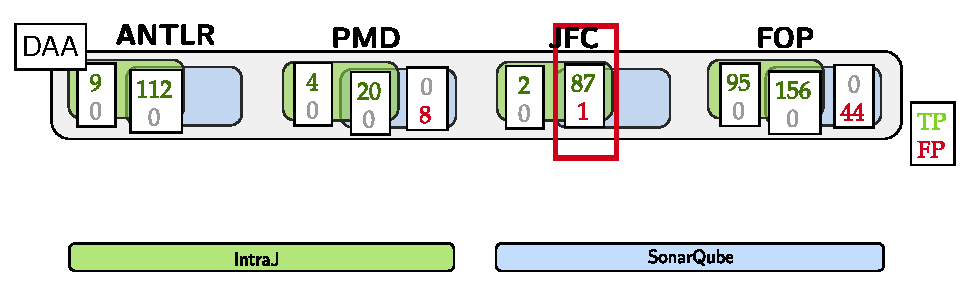
\includegraphics[scale=0.7]{img/precision3.pdf}}
		\only<4>{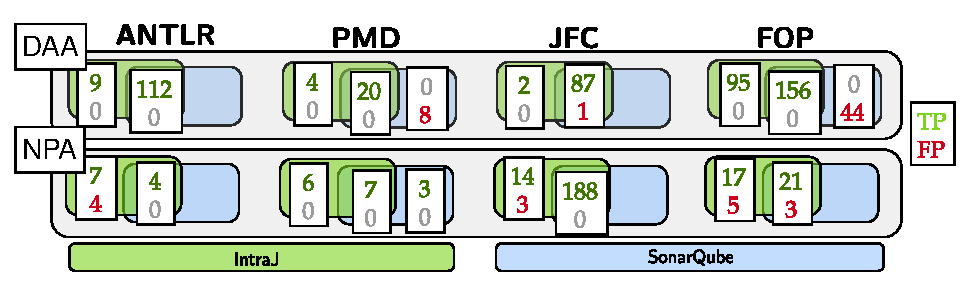
\includegraphics[scale=0.7]{img/precision4.pdf}}
		\only<5->{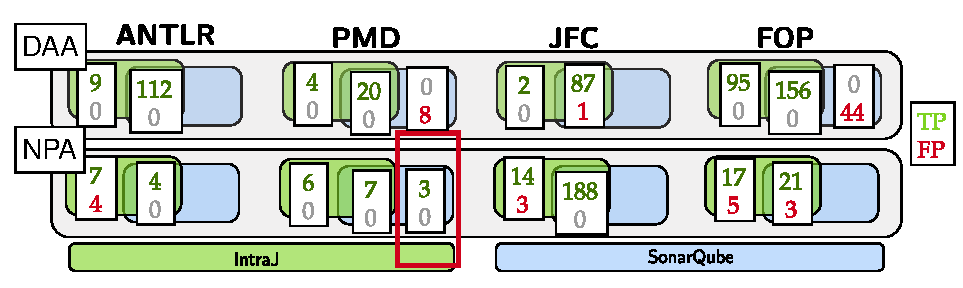
\includegraphics[scale=0.7]{img/precision5.pdf}}


\onslide<6->{
\begin{table}
\centering
\begin{tabular}{|c|r|r|r|r|r|r|}
\hline
\multirow{2}{*}{Benchmark } & \multicolumn{2}{c|}{\textbf{\color<7>{ForestGreen}{Baseline}} (s)}               & \multicolumn{2}{c|}{ \color<8>{ForestGreen}{\textbf{DAA}} (s)}                     & \multicolumn{2}{c|}{\textbf{ \color<9>{ForestGreen}{NPA}} (s)}                     \\
\cline{2-7}
                            & \multicolumn{1}{c|}{IntraJ} & \multicolumn{1}{c|}{SQ} & \multicolumn{1}{c|}{IntraJ} & \multicolumn{1}{c|}{SQ} & \multicolumn{1}{c|}{IntraJ} & \multicolumn{1}{c|}{SQ}  \\
\hline
\textbf{ANTLR}              & \color<7>{ForestGreen}{2.14}                        &  \color<7>{red}{4.91}                    &  \color<8>{red}{0.53}                        & \color<8>{ForestGreen}{0.24}                   &  \color<9>{ForestGreen}{0.90}                             &  \color<9>{red}{12.35}                    \\
\hline
\textbf{PMD}                &  \color<7>{ForestGreen}{3.56}                     & \color<7>{red}{10.76}                  &  \color<8>{red}{0.47}                        &  \color<8>{ForestGreen}{0.18}                   &  \color<9>{ForestGreen}{0.80}                        &   \color<9>{red}{12.40}                    \\
\hline
\textbf{JFC}                &  \color<7>{ForestGreen}{4.29}                       &\color<7>{red}{10.81}                &  \color<8>{red}{0.75}                        &  \color<8>{ForestGreen}{0.24}                    &  \color<9>{ForestGreen}{1.62}                        &   \color<9>{red}{10.71}                    \\
\hline
\textbf{FOP}                &  \color<7>{ForestGreen}{ 4.42}                     & \color<7>{red}{17.20}                  &  \color<8>{red}{0.67}                       &  \color<8>{ForestGreen}{0.34}                    &  \color<9>{ForestGreen}{1.42}                        &   \color<9>{red}{19.25}                    \\
\hline
\end{tabular}
\end{table}
}
\end{frame}




%    \begin{minipage}{0.4\textwidth}
%    \begin{lstlisting}[ language=Java, label=listing:npaTruePositiveIntraJ, basicstyle=\tiny]
%void bar(boolean flag){
%  Object o = null;
%  if (flag)
%    o = new Object();
%  if (flag)
%    println(o.toString());
%}
%    \end{lstlisting}
%    \end{minipage}%
%	\hfill
%    \begin{minipage}{0.4\textwidth}
%    \begin{lstlisting}[ language=Java, label=listing:npaTruePositiveSQ, basicstyle=\tiny]
%void foo(){
%  Object rs = getRS();
%  if(rs==null)
%      // rs can be null
%      panic(); //exit(1)
%  println(rs.toString());
%}
%    \end{lstlisting}
%    \end{minipage}%\